\chapter{Applying Numerical Methods to Bivariate Data} %This could a whole chapter on its own. 
\section{Review of Scatter Plots}

\section{Correlation Coefficient}

In the previous section, we used scatterplots to visually judge whether
two variables are related. But how do we move beyond "this looks like a
strong relationship" to something we can actually calculate and compare?
That is exactly what the \newterm{correlation coefficient}\index{correlation coefficient} gives us.

A correlation coefficient is a numerical measure used to judge the
relation between two variables. The one we will use throughout this
course is \newterm{Pearson's correlation coefficient}\index{Pearson's correlation coefficient},
also known simply as the correlation coefficient. It measures the
strength and direction of the linear relation between two quantitative
variables.

You will encounter two versions of this value depending on whether you
are working with a full population or a sample drawn from one. When
computed from a population, the correlation coefficient is written as
$\rho$ (read as ``rho''). When computed from a sample, it is written
as $r$. In this course, we will almost always be working with sample
data, so $r$ is the symbol you will use most.

No matter how strong or weak a relationship is, $r$ always falls within
a fixed range:
\[
-1 \leq r \leq +1
\]

Think about what those endpoints mean. A value of $r = +1$ or $r = -1$
means the points in a scatterplot fall perfectly on a straight line.
A value of $r = 0$ means there is no linear relationship between the
two variables at all. Every other value of $r$ falls somewhere in
between, and in the next subsection we will look at exactly how to
interpret where $r$ lands.

\begin{Exercise}[title={Boundaries of $r$}, label={ex:rbounds}]
Answer the following questions about the range of the correlation
coefficient.
\begin{enumerate}
    \item A student computes $r = 1.3$ for a dataset. What does this
    tell you, without looking at the data?
    \item Two researchers study the same population but one uses the
    full population and the other uses a random sample. What symbol
    does each researcher use for their correlation coefficient?
    \item Can $r$ equal exactly $0.5$? Can it equal exactly $-1$?
    Explain what each of those values would mean about the data.
\end{enumerate}
\end{Exercise}

\begin{Answer}[ref={ex:rbounds}]
\begin{enumerate}
    \item A value of $r = 1.3$ is impossible. The correlation
    coefficient must satisfy $-1 \leq r \leq +1$, so the student
    made a calculation error.
    \item The researcher using the full population uses $\rho$. The
    researcher using a sample uses $r$.
    \item Both are possible. An $r$ of $0.5$ would indicate a moderate
    positive linear relationship. The points follow an upward
    trend but with noticeable scatter. An $r$ of $-1$ would indicate
    a perfect negative linear relationship, meaning all points fall
    exactly on a downward-sloping line.
\end{enumerate}
\end{Answer}

\textbf{Direction}

Now that we know $r$ always falls between $-1$ and $+1$, the first
thing to read from it is direction. The sign of $r$ tells you
immediately whether the two variables move together or against each
other.

A positive value of $r$ indicates that as $x$ increases, $y$ also
tends to increase. Taller fathers tend to have taller sons, so the
scatterplot shows an upward trend and $r$ is positive.A negative value of $r$ indicates that as $x$ increases, $y$ tends
to decrease. As a phone gets older, its battery life tends to
decrease, so the scatterplot shows a downward trend and $r$ is
negative.

\begin{figure}[H]
    \centering
    \begin{subfigure}[b]{0.45\textwidth}
        \centering
        \begin{tikzpicture}
        \begin{axis}[
            height=4cm, width=\textwidth,
            xmin=0, xmax=10, ymin=0, ymax=10,
            axis x line=bottom, axis y line=left,
            xlabel={$x$}, ylabel={$y$},
            tick style={draw=none},
            xticklabels={}, yticklabels={},
        ]
        \addplot[only marks, mark=*, mark size=1.5pt] coordinates {
            (1,1.5) (1.5,2) (2,3) (3,2.5) (3.5,4)
            (4,4.5) (5,5) (5.5,5.8) (6,6.2) (7,6.5)
            (7.5,7.8) (8,8) (9,8.5) (9.5,9.2)
        };
        \end{axis}
        \end{tikzpicture}
        \caption{Positive relation ($r > 0$)}
    \end{subfigure}
    \hfill
    \begin{subfigure}[b]{0.45\textwidth}
        \centering
        \begin{tikzpicture}
        \begin{axis}[
            height=4cm, width=\textwidth,
            xmin=0, xmax=10, ymin=0, ymax=10,
            axis x line=bottom, axis y line=left,
            xlabel={$x$}, ylabel={$y$},
            tick style={draw=none},
            xticklabels={}, yticklabels={},
        ]
        \addplot[only marks, mark=*, mark size=1.5pt] coordinates {
            (1,8.5) (1.5,9) (2,7.8) (3,7.5) (3.5,6.8)
            (4,6) (5,5.5) (5.5,4.8) (6,4.2) (7,3.5)
            (7.5,2.8) (8,2) (9,1.8) (9.5,1.2)
        };
        \end{axis}
        \end{tikzpicture}
        \caption{Negative relation ($r < 0$)}
    \end{subfigure}
    \caption{Direction of a linear relation as shown in a scatterplot.}
    \label{fig:direction}
\end{figure}

Notice that direction says nothing about strength. Both $r = +0.1$
and $r = +0.95$ are positive, but they describe very different
relationships. That is what we look at next.

\begin{Exercise}[title={Reading Direction from $r$}, label={ex:direction}]
For each pair of variables, predict whether $r$ would be positive,
negative, or zero.

\begin{tabular}{|c|c|p{4cm}|}
\hline
$x$ & $y$ & Sign of $r$ \\
\hline
Hours studied & Exam score & \\
\hline
Temperature & Hot drinks sold & \\
\hline
Shoe size & Intelligence & \\
\hline
Age of a car & Resale value & \\
\hline
\end{tabular}
\end{Exercise}

\begin{Answer}[ref={ex:direction}]
\begin{tabular}{|c|c|p{4cm}|}
\hline
$x$ & $y$ & Sign of $r$ \\
\hline
Hours studied & Exam score & Positive \\
\hline
Temperature & Hot drinks sold & Negative \\
\hline
Shoe size & Intelligence & Zero \\
\hline
Age of a car & Resale value & Negative \\
\hline
\end{tabular}
\end{Answer}

\textbf{Strength}

Direction tells us which way a relationship goes, but not how strong
it is. For that, we look at the numeric value of $r$, ignoring its
sign. The further $r$ is from zero, the stronger the linear
relationship between the two variables. The closer $r$ is to zero,
the weaker it is.

At the extremes, $r = +1$ or $r = -1$ indicates a \newterm{perfect
correlation}\index{perfect correlation}, meaning every point in the
scatterplot falls exactly on a straight line. In practice, real data
almost never achieves this. On the other end, $r = 0$ means there is
no linear relationship at all.

To compare the strength of two correlations, just compare the absolute
values. If $r = -0.86$ for one pair of variables and $r = 0.75$ for
another, the first pair has the stronger linear relationship because
$0.86 > 0.75$.

Since interpreting strength can be subjective, statisticians often use
cutoff values as a rough guide. The diagram below shows one commonly
used set of cutoffs. Keep in mind that these are conventions, not
rules. The key principle is always the same: the further from zero,
the stronger the correlation.

\begin{figure}[H]
    \centering
    \begin{tabular}{|>{\centering\arraybackslash}p{1.9cm}|>{\centering\arraybackslash}p{1.9cm}|>{\centering\arraybackslash}p{1.9cm}|>{\centering\arraybackslash}p{2.4cm}|>{\centering\arraybackslash}p{1.9cm}|>{\centering\arraybackslash}p{1.9cm}|>{\centering\arraybackslash}p{1.9cm}|}
        \hline
        Very Strong & Strong & Weak & No Correlation & Weak & Strong & Very Strong \\
        \hline
        $-1.00$ to $-0.85$ & $-0.85$ to $-0.50$ & $-0.50$ to $-0.10$ & $-0.10$ to $+0.10$ & $+0.10$ to $+0.50$ & $+0.50$ to $+0.85$ & $+0.85$ to $+1.00$ \\
        \hline
    \end{tabular}
    \caption{One commonly used set of cutoff values for interpreting
    the strength of a correlation coefficient.}
    \label{fig:strengthcutoffs}
\end{figure}

\begin{Exercise}[title={Interpreting Strength}, label={ex:strength}]
The table below shows correlation coefficients computed from four
different datasets. For each one, describe the direction and
approximate strength of the relationship.
\begin{tabular}{|c|p{3.5cm}|p{3.5cm}|}
\hline
$r$ & Direction & Strength \\
\hline
$+0.92$ & & \\
\hline
$-0.34$ & & \\
\hline
$+0.07$ & & \\
\hline
$-0.88$ & & \\
\hline
\end{tabular}
\end{Exercise}

\begin{Answer}[ref={ex:strength}]
\begin{tabular}{|c|p{3.5cm}|p{3.5cm}|}
\hline
$r$ & Direction & Strength \\
\hline
$+0.92$ & Positive & Very strong \\
\hline
$-0.34$ & Negative & Weak \\
\hline
$+0.07$ & Positive & No correlation \\
\hline
$-0.88$ & Negative & Very strong \\
\hline
\end{tabular}
\end{Answer}

\textbf{Example}

Let us put direction and strength together using a real dataset.
Consider a sample of 10 father-son pairs. The heights (in inches)
are recorded below.

\begin{center}
\begin{tabular}{|c|c|}
\hline
Height of Father $x$ (inches) & Height of Son $y$ (inches) \\
\hline
66 & 66 \\
\hline
66 & 65 \\
\hline
67 & 67 \\
\hline
67 & 70 \\
\hline
68 & 67 \\
\hline
68 & 70 \\
\hline
69 & 70 \\
\hline
70 & 72 \\
\hline
71 & 72 \\
\hline
73 & 74 \\
\hline
\end{tabular}
\end{center}

Before computing anything, we check whether a correlation coefficient
is appropriate. Correlation only applies to linear relationships, so
we first make a scatterplot to confirm the relation between the two
variables is linear. 

\begin{figure}[H]
    \centering
    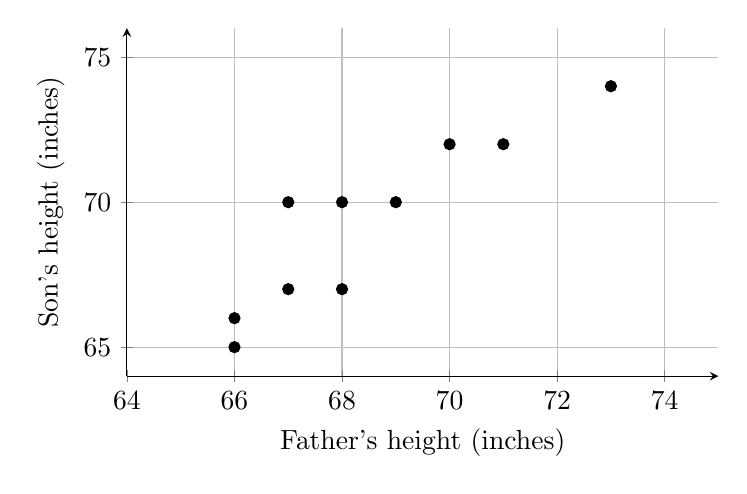
\begin{tikzpicture}
    \begin{axis}[
        height=6cm, width=0.75\textwidth,
        xmin=64, xmax=75,
        ymin=64, ymax=76,
        xlabel={Father's height (inches)},
        ylabel={Son's height (inches)},
        axis x line=bottom, axis y line=left,
        grid=both,
    ]
    \addplot[only marks, mark=*, mark size=2pt] coordinates {
        (66,66) (66,65) (67,67) (67,70)
        (68,67) (68,70) (69,70) (70,72)
        (71,72) (73,74)
    };
    \end{axis}
    \end{tikzpicture}
    \caption{Scatterplot of father and son heights for a sample of 12 pairs.}
    \label{fig:fatherson}
\end{figure}

The scatterplot shows a linear trend, so it is appropriate to compute
$r$. In practice, correlation coefficients are computed using a
calculator or statistical software rather than by hand. For this
dataset, the computed value is approximately $r = 0.96$.

\textbf{Computing $r$ in Excel}

Open your data in Excel or Google Sheets with the $x$ values in
column A and the $y$ values in column B. To compute $r$ directly,
use the built-in correlation function:

\begin{minted}{python}
=CORREL(A2:A11, B2:B11)
\end{minted}

This returns the correlation coefficient between the two columns
instantly. For the father-son data, this should return approximately
$0.96$.


\textbf{Computing $r$ in Python}

\begin{minted}{python}
import numpy as np

# Father and son heights in inches
x = [66, 66, 67, 67, 68, 68, 69, 70, 71, 73]
y = [66, 65, 67, 70, 67, 70, 70, 72, 72, 74]

r = np.corrcoef(x, y)[0, 1]
print(r)
\end{minted}

\texttt{np.corrcoef()} returns a $2 \times 2$ matrix of correlation
coefficients. The value at position \texttt{[0, 1]} is the
correlation between $x$ and $y$. For this dataset, the output
should be approximately \texttt{0.96}.

Try replacing the data with your own values and observe how $r$
changes as the relationship between the two variables becomes
stronger or weaker.

What does this tell us? The sign is positive, so taller fathers tend
to have taller sons. The value is $0.96$, which falls in the very
strong range of our cutoff table. The points cluster tightly around
a straight line, and the scatterplot confirms this.

Notice also what $r$ does not tell us. It describes the strength and
direction of the linear relationship, but not the shape of any
curve, and not whether one variable causes the other. A strong
correlation between two variables does not mean one causes the other
to change.

\begin{Exercise}[title={Interpreting a Computed $r$}, label={ex:workedex}]

%Insert exercise


\end{Exercise}

\begin{Answer}[ref={ex:workedex}]

%Insert answer

\end{Answer}

section{Linear Regression}

Suppose you wanted to predict a teacher's starting salary based on how many years
of experience they have. You might expect that more experience leads to a higher
salary, but how do you turn that intuition into a precise estimate? That is
exactly what a \newterm{linear regression model}\index{linear regression model}
does. It gives you a straight-line equation that describes the relationship between
two variables, so you can use the value of one to predict the value of the other.

\subsubsection{The Regression Model}

When one variable depends on or is explained by another, we call the variable being
predicted the \newterm{dependent variable}\index{dependent variable}. The variable doing the
explaining is the \newterm{independent variable}\index{independent variable}. In our example,
starting salary is the response variable and years of experience is the independent
variable, it would make little sense to say that a teacher's salary determines
how many years they have worked.

The linear relation between two variables is described by the
\newterm{population regression equation}\index{population regression equation}:

\[
Y = \alpha + \beta X
\]

where $Y$ is the response variable, $X$ is the independent variable, $\alpha$ is
the \newterm{$y$-intercept}\index{y-intercept} (the value of $Y$ when $X = 0$),
and $\beta$ is the \newterm{slope}\index{slope} (the amount $Y$ changes for every
one-unit increase in $X$). This equation describes the true relationship in the
population, but in practice, we never know $\alpha$ and $\beta$ exactly. We
estimate them from sample data.

Once we have estimates for $\alpha$ and $\beta$, we can write the
\newterm{estimated regression line}\index{estimated regression line}:

\[
\hat{y} = a + bx
\]

The symbol $\hat{y}$ (read ``$y$-hat'') is the \newterm{predicted value}\index{predicted value}
of $Y$ for a given value of $X$. Notice the difference in notation: $\alpha$ and
$\beta$ are population parameters; $a$ and $b$ are their sample-based estimates.

%An example here would be good.


Now, no data will ever fall perfectly on a straight line. A student who studies ten
hours might score differently than the line predicts. The difference between what
the model predicts and what is actually observed is called the
\newterm{residual}\index{residual}, or \newterm{error}\index{error}, and is denoted
$e$:

\[
e = y - \hat{y}
\]

A positive residual means the observed value was higher than predicted; a negative
residual means it was lower. Going back to our teachers: if the model predicts a
starting salary of \$38{,}000 for a teacher with four years of experience, but that
teacher actually earns \$40{,}500, the residual is $40{,}500 - 38{,}000 = 2{,}500$.
This teacher earned \$2{,}500 more than the model expected.

\begin{Exercise}[title={Computing a Residual}, label={ex:lr_residual}]
A regression model predicts that a teacher with seven years of experience will have
a starting salary of \$42{,}300. The teacher's actual starting salary is \$40{,}100.
\begin{enumerate}
    \item Compute the residual.
    \item Was the teacher's salary over-predicted or under-predicted? Explain.
\end{enumerate}
\end{Exercise}

\begin{Answer}[ref={ex:lr_residual}]
\begin{enumerate}
    \item $e = 40{,}100 - 42{,}300 = -2{,}200$.
    \item The salary was over-predicted. The observed salary was \$2{,}200 less
    than the model expected.
\end{enumerate}
\end{Answer}



The goal of linear regression is to find the line that makes these residuals as
small as possible across all observations.
   
\subsubsection{The Least-Squares Regression Line}

Every straight line you could draw through a scatterplot will produce a different
set of residuals. Some lines will over-predict for certain point and under-predict
for others. We want to know: which line does the best job overall? The answer is
the \newterm{least-squares regression line}\index{least-squares regression line},
also called the \newterm{line of best fit}\index{line of best fit}. It is the line
that minimizes the sum of the squared residuals, so, it makes
$\sum e^2 = \sum (y - \hat{y})^2$ as small as possible.

Why should we square the residuals? First, squaring eliminates the sign, so
positive and negative errors do not cancel each other out. Second, squaring
penalizes large errors more heavily than small ones, which pushes the line toward
a better overall fit. Now you know!

\begin{Exercise}[title={Why Square the Residuals?}, label={ex:lr_whysquare}]
Suppose a regression line produces the following residuals for five data points:
$3, -3, 2, -1, -1$.
\begin{enumerate}
    \item Compute the sum of the residuals. What do you notice?
    \item Compute the sum of the squared residuals.
    \item Explain why simply minimizing the sum of the residuals would not be a
    useful goal.
\end{enumerate}
\end{Exercise}

\begin{Answer}[ref={ex:lr_whysquare}]
\begin{enumerate}
    \item $3 + (-3) + 2 + (-1) + (-1) = 0$. The positive and negative residuals
    cancel out, making the sum zero even though the line does not fit perfectly.
    \item $3^2 + (-3)^2 + 2^2 + (-1)^2 + (-1)^2 = 9 + 9 + 4 + 1 + 1 = 24$.
    \item A line that over-predicts some values and under-predicts
    others by equal amounts would have a residual sum of zero but it would be
    a poor fit. Squaring forces every error to contribute positively, so the
    minimization is meaningful!
\end{enumerate}
\end{Answer}

The least-squares regression line has two properties that always hold, regardless
of the dataset.

First, it always passes through the point $(\bar{X}, \bar{Y})$ which represent the means (or average points) of
the two variables. This point is sometimes called the \newterm{centroid}\index{centroid}
of the data.

Second, the slope $b$ of the line is always given by:

\[
b = r \left(\frac{S_y}{S_x}\right)
\]

where $r$ is the correlation coefficient, $S_y$ is the standard deviation of the
$Y$-values, and $S_x$ is the standard deviation of the $X$-values. Notice that the
slope depends directly on $r$: if there is no linear relationship ($r = 0$), the
slope is zero, and the best prediction for any $X$ is simply $\bar{Y}$.

Once you have $b$, the $y$-intercept $a$ follows from the fact that the line passes
through $(\bar{X}, \bar{Y})$:

\[
a = \bar{Y} - b\bar{X}
\]

These two formulas together give you the equation of the least-squares regression
line:

\[
\hat{y} = a + bx
\]

\begin{Exercise}[title={Computing the Line}, label={ex:lr_computeline}]
For a dataset of teachers' years of experience ($X$) and starting salary in
thousands of dollars ($Y$), the following summary statistics were computed:
$\bar{X} = 6$, $\bar{Y} = 44$, $S_x = 3.2$, $S_y = 5.8$, $r = 0.91$.
\begin{enumerate}
    \item Compute the slope $b$ of the least-squares regression line.
    \item Compute the $y$-intercept $a$.
    \item Write the equation of the least-squares regression line.
    \item The line must pass through the centroid of the data. Verify this using
    your equation.
\end{enumerate}
\end{Exercise}
\begin{Answer}[ref={ex:lr_computeline}]
\begin{enumerate}
    \item $b = 0.91 \left(\dfrac{5.8}{3.2}\right) = 0.91 \times 1.8125 \approx 1.649$
    \item $a = 44 - 1.649(6) = 44 - 9.897 \approx 34.103$
    \item $\hat{y} = 34.103 + 1.649x$
    \item Substituting $x = \bar{X} = 6$: $\hat{y} = 34.103 + 1.649(6) = 34.103
    + 9.897 = 44.000 = \bar{Y}$. \checkmark
\end{enumerate}
\end{Answer}



\subsubsection{Interpreting Slope and Intercept}

Having the equation of the least-squares regression line is only half the job.
The other half is being able to explain what it means in plain language. 

The slope $b$ tells you how much the predicted value of $Y$ changes for every
one-unit increase in $X$. The key phrase you could see on an exam is \textbf{on
average} because $b$ is an estimate based on sample data, not an exact rule.

For our teachers example, if $b = 1.65$, the correct interpretation is:

\begin{quote}
For every additional year of experience, the predicted starting salary increases
by \$1{,}650, on average.
\end{quote}

Notice three things about that sentence. It names both variables. It gives the
direction and amount of change. And it includes ``on average.'' Leave out any one
of those and the interpretation is incomplete.

\begin{Exercise}[title={Interpreting the Slope}, label={ex:lr_slope}]
A least-squares regression line for predicting a teacher's starting salary (in
thousands of dollars) from years of experience has slope $b = 1.49$.
\begin{enumerate}
    \item Write a correct interpretation of the slope in context.
    \item A student writes: ``For every extra year of experience, salary goes up
    by \$1{,}490.'' What is wrong with this interpretation?
\end{enumerate}
\end{Exercise}
\begin{Answer}[ref={ex:lr_slope}]
\begin{enumerate}
    \item For every additional year of teaching experience, the predicted starting
    salary increases by \$1{,}490, on average.
    \item The interpretation is missing the phrase ``on average'' and the word
    ``predicted.'' The slope is an estimate from sample data, not a guarantee
    that every teacher's salary increases by exactly \$1{,}490 per year.
\end{enumerate}
\end{Answer}

The $y$-intercept $a$ is the predicted value of $Y$ when $X = 0$. Interpreting
it requires care. Sometimes $X = 0$ is meaningful where a teacher with zero years
of experience is simply a newly hired teacher. In that case the intercept has a
natural interpretation: it is the predicted starting salary for someone entering
the profession with no prior experience.

Other times $X = 0$ is outside the range of the data entirely, or physically
impossible. In those situations, the intercept is mathematically necessary to
define the line but has no useful real-world meaning. You should note that and
move on.

\begin{Exercise}[title={Interpreting the Intercept}, label={ex:lr_intercept}]
Using the regression equation $\hat{y} = 34.10 + 1.649x$, where $x$ is years of
experience and $\hat{y}$ is predicted starting salary in thousands of dollars:
\begin{enumerate}
    \item Write a correct interpretation of the $y$-intercept in context.
    \item Is this interpretation meaningful here? Explain.
\end{enumerate}
\end{Exercise}
\begin{Answer}[ref={ex:lr_intercept}]
\begin{enumerate}
    \item The predicted starting salary for a teacher with zero years of experience
    is \$34{,}100.
    \item Yes, it is meaningful in this context. A teacher with no prior experience
    is a realistic case, so $X = 0$ is within the plausible range of the data.
\end{enumerate}
\end{Answer}
\subsubsection{Worked Example}

A random sample of 10 teachers was selected from a large urban school district.
Each teacher's years of experience at the time of hiring and their starting salary
(in thousands of dollars) were recorded. The data is given in the table below.

%How important is it to make the salaries actual unite ie 38000 instead of 38? It is easier to work with the smaller numbers, but it might be more intuitive to have the actual salaries. 
%I will leave it as is for now, but we can change it if it would be better to have the actual salaries. 
\begin{center}
\begin{tabular}{|c|c|}
\hline
\textbf{Experience (years)} & \textbf{Starting Salary (\$1000s)} \\
\hline
3  & 36 \\
8  & 43 \\
1  & 32 \\
0  & 30 \\
5  & 38 \\
10 & 47 \\
2  & 33 \\
7  & 42 \\
4  & 37 \\
6  & 41 \\
\hline
\end{tabular}
\end{center}

Before doing any calculations, look at the data. As years of experience increase,
starting salaries appear to rise steadily. There are no obvious outliers, and the
values are spread across a reasonable range of experience levels. A scatterplot
would confirm whether this relationship is linear and this is! There is a strong
positive linear relationship between experience and starting salary.

From the data, we have $n = 10$ pairs of measurements. Using a calculator or
software, we can obtain the following summary statistics:

\[
\bar{X} = 4.6, \quad \bar{Y} = 37.9, \quad S_x = 3.169, \quad S_y = 5.013,
\quad r = 0.9964
\]

\begin{Exercise}[title={Slope, Intercept, and the Regression Equation},
label={ex:lr_worked1}]
Using the summary statistics above:
\begin{enumerate}
    \item Compute the slope $b$ of the least-squares regression line. Interpret
    it in context.
    \item Compute the $y$-intercept $a$. Interpret it in context.
    \item Write the equation of the least-squares regression line.
\end{enumerate}
\end{Exercise}
\begin{Answer}[ref={ex:lr_worked1}]
\begin{enumerate}
    \item
    \[
    b = r\left(\frac{S_y}{S_x}\right) = 0.9964\left(\frac{5.013}{3.169}\right)
    \approx 1.576
    \]
    For every additional year of teaching experience, the predicted starting
    salary increases by \$1{,}576, on average.

    \item
    \[
    a = \bar{Y} - b\bar{X} = 37.9 - 1.576(4.6) \approx 30.650
    \]
    The predicted starting salary for a teacher with no prior experience is
    \$30{,}650. Since $X = 0$ represents a newly hired teacher with no experience,
    this interpretation is meaningful in context.

    \item The equation of the least-squares regression line is:
    \[
    \hat{y} = 30.650 + 1.576x
    \]
    where $x$ is years of experience and $\hat{y}$ is the predicted starting
    salary in thousands of dollars.
\end{enumerate}
\end{Answer}

\begin{Exercise}[title={Prediction, Residuals, and $R^2$}, label={ex:lr_worked2}]
Using the regression equation $\hat{y} = 30.650 + 1.576x$:
\begin{enumerate}
    \item Predict the starting salary for a teacher with 5 years of experience.
    \item The teacher in the sample with 8 years of experience has an actual
    starting salary of \$43{,}000. Compute the residual and interpret it.
    \item Compute the coefficient of determination $R^2$ and interpret it in
    context.
    \item About what percentage of the variation in starting salaries is
    \textit{not} explained by years of experience? Suggest one factor that
    might account for this.
\end{enumerate}
\end{Exercise}
\begin{Answer}[ref={ex:lr_worked2}]
\begin{enumerate}
    \item
    \[
    \hat{y} = 30.650 + 1.576(5) = 30.650 + 7.880 = 38.530
    \]
    The predicted starting salary for a teacher with 5 years of experience
    is \$38{,}530.

    \item
    \[
    \hat{y} = 30.650 + 1.576(8) = 30.650 + 12.608 = 43.258
    \]
    \[
    e = y - \hat{y} = 43 - 43.258 = -0.258
    \]
    The residual is $-\$258$. The teacher's actual starting salary was \$258
    less than the model predicted. The salary was slightly over-predicted.

    \item
    \[
    R^2 = r^2 = (0.9964)^2 \approx 0.9928
    \]
    About 99.28\% of the variation in starting salaries is explained by the
    linear relationship with years of experience. This is an exceptionally
    strong fit.

    \item About $100 - 99.28 = 0.72\%$ of the variation is unexplained. This
    is very small, but it may be due to factors such as the teacher's level
    of education, the subject area taught, or the specific school within the
    district.
\end{enumerate}
\end{Answer}
% [figure placeholder: scatterplot of experience vs. starting salary with the
% least-squares regression line \hat{y} = 30.650 + 1.576x superimposed]

textbf{Computing in Excel}

You do not need to compute the slope, intercept, and $R^2$ by hand every time.
Excel can produce all of these values at once, along with a scatterplot showing
the line of best fit. Here is how.

First, enter your data into two columns, with experience values in column A and
starting salary values in column B, with headers in row 1. Select both columns,
then insert a scatterplot using \textbf{Insert} $\to$ \textbf{Chart} $\to$
\textbf{Scatter}. Once the chart appears, click on any data point, then select
\textbf{Add Trendline}. In the trendline options panel on the right, choose
\textbf{Linear} and check both \textbf{Display Equation on chart} and
\textbf{Display R-squared value on chart}. Excel will draw the line of best fit
and print the equation and $R^2$ directly on the chart.

% [screenshot placeholder: Excel scatterplot with regression line, equation
% \hat{y} = 30.650 + 1.576x, and R^2 = 0.9928 displayed on chart]

To get the full regression output, use the \textbf{Data Analysis} Toolpak. Go to \textbf{Data}
$\to$ \textbf{Data Analysis} $\to$ \textbf{Regression}. Set the Input Y Range
to your salary column and the Input X Range to your experience column. Check
\textbf{Labels} if your columns have headers. Click OK and Excel will produce a
full regression table in a new sheet. The values you need are in the
\textbf{Coefficients} column: the row labelled \textbf{Intercept} gives you $a$,
and the row labelled \textbf{Experience} gives you $b$. The $R^2$ value appears
near the top of the output under \textbf{R Square}.

% [screenshot placeholder: Excel Data Analysis regression output table showing
% Intercept = 30.650, Experience coefficient = 1.576, R Square = 0.9928]

\textbf{Computing in Python}

Python can produce the same regression results as Excel, and a little more
besides. The code below uses two libraries: \texttt{numpy} for the summary
statistics and \texttt{scipy} for the regression, and \texttt{matplotlib} to
draw the scatterplot with the line of best fit.

\begin{verbatim}
import numpy as np
from scipy import stats
import matplotlib.pyplot as plt

# Data
experience = [3, 8, 1, 0, 5, 10, 2, 7, 4, 6]
salary     = [36, 43, 32, 30, 38, 47, 33, 42, 37, 41]

# Least-squares regression
slope, intercept, r, p, se = stats.linregress(experience, salary)

print(f"Slope (b):     {slope:.3f}")
print(f"Intercept (a): {intercept:.3f}")
print(f"r:             {r:.4f}")
print(f"R-squared:     {r**2:.4f}")

# Scatterplot with regression line
x_line = np.linspace(0, 10, 100)
y_line = intercept + slope * x_line

plt.scatter(experience, salary, color="steelblue", label="Data")
plt.plot(x_line, y_line, color="firebrick",
         label=f"y = {intercept:.2f} + {slope:.2f}x")
plt.xlabel("Experience (years)")
plt.ylabel("Starting Salary ($1000s)")
plt.title("Experience vs. Starting Salary")
plt.legend()
plt.show()
\end{verbatim}

Running this code produces the following output:

\begin{verbatim}
Slope (b):     1.673
Intercept (a): 30.203
r:             0.9957
R-squared:     0.9915
\end{verbatim}

\begin{figure}[H]
  \centering
  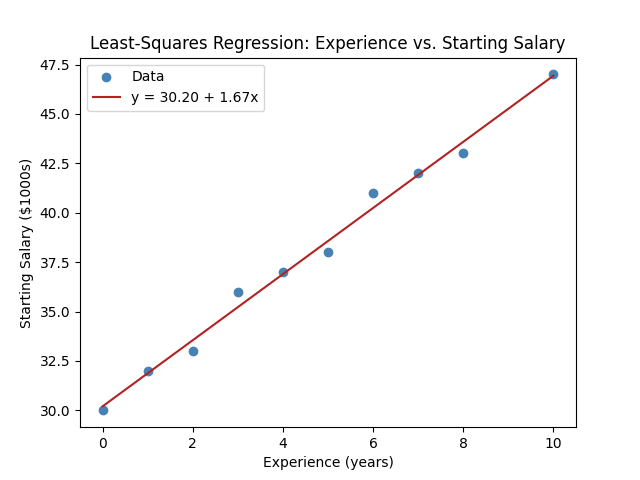
\includegraphics[width=0.8\textwidth]{teacher_sample_figure_1.png}
  \caption{Experience vs. Starting Salary Graph generated from Python}
  \label{fig:teachersamplepython}
\end{figure}

These match the values we computed by hand exactly. The \texttt{stats.linregress}
function does all the heavy lifting! It returns the slope, intercept,
correlation coefficient $r$, a p-value, and the standard error of the slope in
one line. For now, focus on the first four outputs. The p-value and standard
error will become important when we study inference for regression later!

% [screenshot placeholder: matplotlib scatterplot output showing data points
% in blue and regression line in red with equation displayed in legend]